\begin{figure}[ht!]
    \centering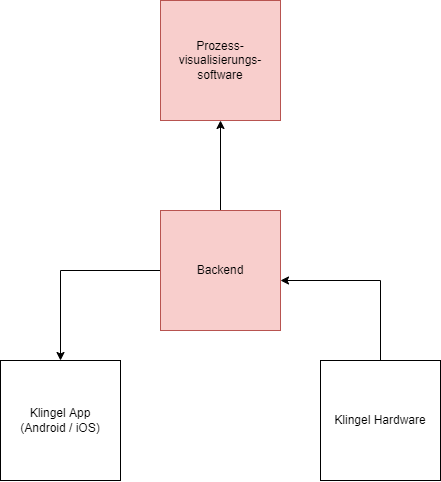
\includegraphics[width=\paperwidth/2]{../assets/img/kontextmodell}

    \caption{Kontextmodell der neu zu entwickelnden Komponenten (Weiß) in Verbindung zu bestehenden Komponenten (Rot)}
    \label{fig:kontextmodell}
\end{figure}
In Abbildung~\ref{fig:kontextmodell} ist das Kontextmodell dargestellt.
Hinzugefügt werden Apps für Android sowie iOS Apps und die Hardware für die Klingel.
Diese werden an das vorhandene Backend angebunden, welches entsprechend erweitert wird.


Die Prozess-visualisierungs-software ist dabei die vorhandene TEKLOTH Software.
Hier müssen die Kameras und Fluss definition für Anrufe und die Konfiguration des Systems im Allgemeinen geschehen.


Das Backend ist das existierende Backend der Prozess-visualisierungs-software und soll um die benannte REST Schnittstellen erweitert werden.
Hier werden auch die Streams und das SIP Protokoll eingebunden.
Auch werden Push benachrichtigungen hier ausgelöst.


Die App ist eine App zur bedienung der Klingelanlage durch Privatnutzer, primär Wohnungsbesitzer.
Sie wird mit einem Cross--Platform Framework umgesetzt und ist deshalb lediglich ein Modul.


Die Klingelhardware ist eine speziell entworfene Hardwarekomponente.
Für sie wird es zwei Projekte geben, die tatsächliche Hardware und die Software für diese.
